\documentclass[../../main]{subfiles}
\begin{document}

\begin{figure}[h!]
\[
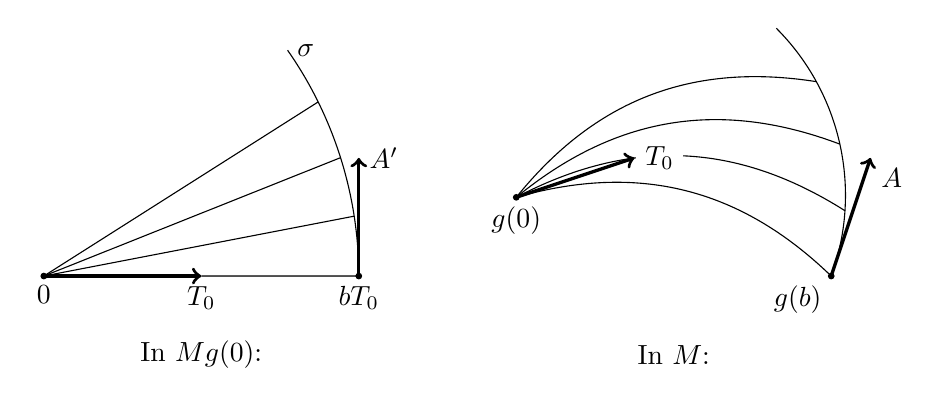
\begin{tikzpicture}
    \begin{scope}
    \filldraw (0,0) circle (1pt) node[anchor=north] {$0$};
    \draw[very thick, ->] (0,0)--(2,0) node[anchor=north] {$T_0$};
    \filldraw (2,0)--(4,0) circle (1pt) node[anchor=north] {$bT_0$};
    \draw[very thick, ->] (4,0)--(4,1.5) node[anchor=west] {$A'$};
    
    \draw (4,0) arc (0:35:5cm)
        coordinate[pos=0.25](P1)
        coordinate[pos=0.5](P2)
        coordinate[pos=0.75](P3)
        node[anchor=west] {$\sigma$};

    \foreach \i in {1,2,3}
    {
        \draw (0,0)--(P\i);
    }
    \end{scope}
    
    \begin{scope}[shift={(6,1)}]
    \filldraw (0,0) circle (1pt) node[anchor=north]{$g(0)$};
    \filldraw (4,-1) circle (1pt) node[anchor=north east]{$g(b)$};
    
    \draw (0,0) to[bend left] (4,-1);
        
    \draw (4,-1) arc (-20:45:3cm)
        coordinate[pos=0.25](P1)
        coordinate[pos=0.5](P2)
        coordinate[pos=0.75](P3);
        
    \foreach \i in {1,2,3}
    {
        \draw (0,0) to[bend left=30] (P\i);
    }
    
    \draw[very thick, ->]
        (0,0)--(1.5,0.5) node[anchor=west, fill=white] {$T_0$};
    \draw[very thick, ->]
        (4,-1)--(4.5,0.5) node[anchor=north west] {$A$};
    \end{scope}
    
    \draw (2,-1) node {In $\tangentspace{M}{g(0)}$:};
    \draw (8,-1) node {In $M$:};
\end{tikzpicture}
\]
\caption{Comparing Geodesics}
\label{fig:ch10fig3}
\end{figure}

\end{document}